\documentclass{article}

\usepackage{amsmath, amsfonts, microtype, xcolor, tikz, graphicx, hyperref, amsthm}
\usepackage[ruled, linesnumbered]{algorithm2e}
\usepackage[]{neurips_2019}

\newtheorem{theorem}{Theorem}

\SetKwComment{Comment}{$\triangleright$\ }{}

\usetikzlibrary{calc}

\tikzset{
    ncbar angle/.initial=90,
    ncbar/.style={
        to path=(\tikztostart)
        -- ($(\tikztostart)!#1!\pgfkeysvalueof{/tikz/ncbar angle}:(\tikztotarget)$)
        -- ($(\tikztotarget)!($(\tikztostart)!#1!\pgfkeysvalueof{/tikz/ncbar angle}:(\tikztotarget)$)!\pgfkeysvalueof{/tikz/ncbar angle}:(\tikztostart)$)
        -- (\tikztotarget)
    },
    ncbar/.default=0.5cm,
}

\tikzset{round left paren/.style={ncbar=0.5cm,out=110,in=-110}}
\tikzset{round right paren/.style={ncbar=0.5cm,out=70,in=-70}}

\title{Measuring causal influence with\\ back-to-back regression: the linear case}

\author{%
  Jean-Remi King\\
  CNRS\\
  \texttt{email} \\
  \And
  Fran\c{c}ois Charton\\
  Facebook AI\\
  \texttt{fcharton@fb.com}\\
  \And
  David Lopez-Paz\\
  Facebook AI\\
  \texttt{dlp@fb.com}
  \And
  Maxime Oquab\\
  Facebook AI\\
  \texttt{qas@fb.com}
}

\begin{document}

\maketitle

\begin{abstract}
Identifying causes from observations is at the core of science. This endeavor
is particularly challenging when i) potential factors are difficult to
manipulate individually and ii) observations are complex and multi-dimensional.
To address this issue, we introduce ``Back-to-Back'' regression (B2B), a
method designed to measure, from a set of co-varying factors, the causal
influences that most plausibly account for multidimensional observations. After
proving the consistency of B2B, we show that our method outperforms
least-squares and related regression and cross-decomposition techniques (e.g.
canonical correlation analysis and partial least squares) on two tasks: causal
identification and out-of-distribution prediction. Finally, we apply B2B to
neuroimaging recordings of 102 subjects reading word sequences. The results
show that the early and late brain responses caused by low- and high-level
word features respectively are more easily detected with B2B than with standard forward regression.
% conclude  open
\end{abstract}

\section{Introduction}

Natural sciences are tasked to find, from a set of hypothetical factors, the
minimal subset that suffices to reliably predict novel observations. This
endeavor is impeded by two major challenges.

First, causal and non-causal factors may be numerous and partially correlated.
% In physics,
% for example, one may be challenged to identify whether fusion is caused by a
% change in temperature or a change in pressure, as these two factors may, at
% first, be difficult to manipulate independently. This issue becomes increasingly
% pronounced as the number of potential factors increases.
In neuroscience, for
example, it can be challenging to identify whether word frequency modulates
brain activity during reading. Indeed, the
frequency of words in natural language covaries with other factors such as their
length (short words are more frequent than long words) and their categories
(determinants are more frequent than adverbs)
\citep{kutas2011thirty,pegado2014timing}. Instead of selecting a set of words
that controls for all of these factors simultaneously, it is thus common to use
a \emph{forward} "encoding model", i.e. to fit a linear regression to predict observations
(e.g. brain activity) from a minimal combination of competing factors (e.g.
word length, word frequency), and analytically investigate
the estimated contribution of each factor from the model's coefficients
\citep{friston1994statistical,naselaris2011encoding,weichwald2015causal,
king2018encoding,huth2016natural}.

The second challenge to measuring causal influence is that observations can be
multidimensional.
For example, brain activity is often
recorded with hundreds or thousands of simultaneous measurements via functional
Magnetic Resonance Imaging, magneto-encephalography (MEG) or multiple electro-
physiological probes \citep{friston1994statistical,steinmetz2018challenges}.
The relationship between putative causes and observations is thus often
done by training models in a \emph{backward}
fashion: i.e. from observations to putative causal factors. For example, it is
common to fit a support vector machine across multiple
brain voxels or multiple electrodes to detect the
category of a stimulus independently of common noise sources (e.g. head
movements, eye blink)
\citep{norman2006beyond,cichy2014resolving,
kriegeskorte2008representational, king2018encoding}.

Both \emph{forward} and \emph{backward} modeling have competing benefits and drawbacks.
Specifically, forward modeling disentangles the independent contribution of
correlated factors, but does not combine multidimensional observations. By
contrast, backward modeling combines multiple observations, but does not
disentangle factors that are linearly correlated \citep{weichwald2015causal,
hebart2018deconstructing, king2018encoding}. To combine some of the benefits of forward
and backward modeling, several authors have proposed to use cross-decomposition
techniques such as Partial Least Squares (PLS) and Canonical Correlation
Analysis (CCA) \citep{de2019multiway, bilenko2016pyrcca}. CCA and PLS aim to find, from two sets of
data $X$ and $Y$, the components $H$ and $G$ such that $XH$ and $YG$ are maximally
correlated or maximally covarying respectively.

While CCA and PLS can make use
of multidimensional features and observations, they are not designed
for feature discovery. First, these methods are not not directional: observations
and factors can be assigned to either $X$ or $Y$. Second, these method project $X$
and $Y$ onto a reduced but nonetheless multidimensional space. Third, because
CCA and PLS are based on a generalized eigen decomposition, their resulting
coefficients mix the features of $X$ and $Y$ in a way that makes them notoriously difficult to
interpret \citep{lebart1995statistique}.

Here, we introduce the `back-to-back regression' (B2B), which not only combines
the benefits of forward and backward modeling (Section~\ref{sec:algorithm}), but
can also provide robust, interpretable, unidimensional and unbiased coefficients for
each factor.

After detailing B2B and proving its convergence
(Section~\ref{sec:theorem}), we show with synthetic data that it outperforms
state-of-the-art forward, backward and cross-decomposition techniques in
disentangling causal factors (Section~\ref{sec:experiment_synthetic}). Finally,
we apply B2B to large neuroimaging datasets and reveal that distinct but
linearly-correlated word features lead to distinguishable brain representations
(Section~\ref{sec:experiment_real}).


\section{Back to back regression}
\label{sec:algorithm}


\begin{figure}[t!]
    \centering
    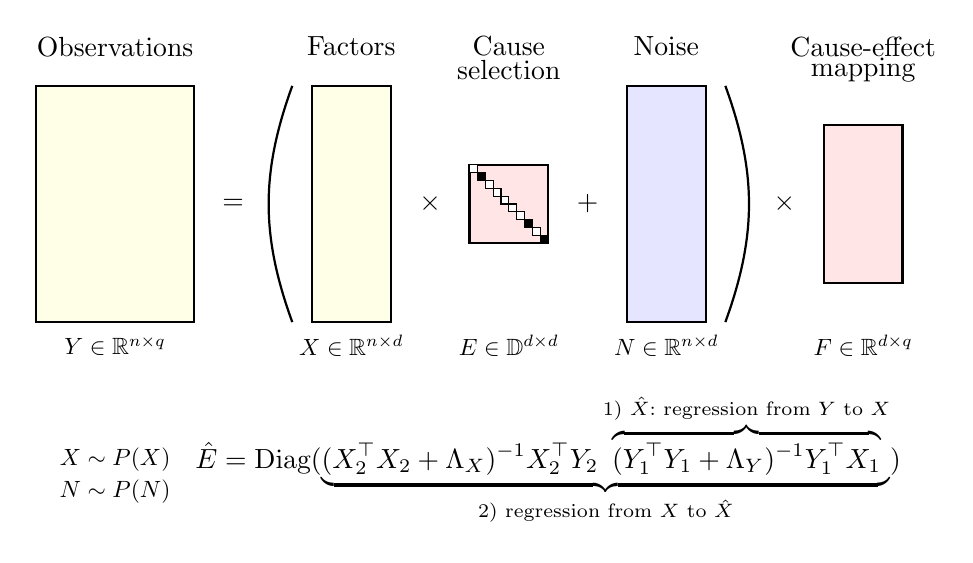
\begin{tikzpicture}
    \newcommand\posY{0}
    \newcommand\posX{3}
    \newcommand\posE{5}
    \newcommand\posN{7}
    \newcommand\posF{9.5}

    \node[thick, draw=black, minimum height=3cm, minimum width=2cm, fill=yellow!10] (Y) at (\posY, 0){};
    \node[] (eq) at (1.5, 0){$=$};
    \node[] (times) at (4, 0){$\times$};
    \node[thick, draw=black, minimum height=3cm, minimum width=1cm, fill=yellow!10] (X) at (\posX, 0){};
    \node[thick, draw=black, minimum height=1cm, minimum width=1cm, fill=red!10] (E) at (\posE, 0){};

    \draw[fill=white] (\posE - 0.5 + 0.0, 0.5 - 0.0) rectangle (\posE - 0.5 + 0.0 + 0.1, 0.5 - 0.0 - 0.1);
    \draw[fill=black] (\posE - 0.5 + 0.1, 0.5 - 0.1) rectangle (\posE - 0.5 + 0.1 + 0.1, 0.5 - 0.1 - 0.1);
    \draw[fill=white] (\posE - 0.5 + 0.2, 0.5 - 0.2) rectangle (\posE - 0.5 + 0.2 + 0.1, 0.5 - 0.2 - 0.1);
    \draw[fill=white] (\posE - 0.5 + 0.3, 0.5 - 0.3) rectangle (\posE - 0.5 + 0.3 + 0.1, 0.5 - 0.3 - 0.1);
    \draw[fill=white] (\posE - 0.5 + 0.4, 0.5 - 0.4) rectangle (\posE - 0.5 + 0.4 + 0.1, 0.5 - 0.4 - 0.1);
    \draw[fill=white] (\posE - 0.5 + 0.5, 0.5 - 0.5) rectangle (\posE - 0.5 + 0.5 + 0.1, 0.5 - 0.5 - 0.1);
    \draw[fill=white] (\posE - 0.5 + 0.6, 0.5 - 0.6) rectangle (\posE - 0.5 + 0.6 + 0.1, 0.5 - 0.6 - 0.1);
    \draw[fill=black] (\posE - 0.5 + 0.7, 0.5 - 0.7) rectangle (\posE - 0.5 + 0.7 + 0.1, 0.5 - 0.7 - 0.1);
    \draw[fill=white] (\posE - 0.5 + 0.8, 0.5 - 0.8) rectangle (\posE - 0.5 + 0.8 + 0.1, 0.5 - 0.8 - 0.1);
    \draw[fill=black] (\posE - 0.5 + 0.9, 0.5 - 0.9) rectangle (\posE - 0.5 + 0.9 + 0.1, 0.5 - 0.9 - 0.1);

    \node[] (plus) at (6, 0){$+$};
    \node[thick, draw=black, minimum height=3cm, minimum width=1cm, fill=blue!10] (N) at (\posN, 0){};
    \node[thick, draw=black, minimum height=2cm, minimum width=1cm, fill=red!10] (F) at (\posF, 0){};
    \draw [thick] (2.25, -1.5) to [round left paren ] (2.25, 1.5);
    \draw [thick] (7.75, -1.5) to [round right paren ] (7.75, 1.5);

    \node[] (times2) at (8.5, 0){$\times$};

    \node[] (annY) at (\posY, -1.8){\scalebox{0.85}{$Y \in \mathbb{R}^{n \times q}$}};
    \node[] (annX) at (\posX, -1.8){\scalebox{0.85}{$X \in \mathbb{R}^{n \times d}$}};
    \node[] (annE) at (\posE, -1.8){\scalebox{0.85}{$E \in \mathbb{D}^{d \times d}$}};
    \node[] (annN) at (\posN, -1.8){\scalebox{0.85}{$N \in \mathbb{R}^{n \times d}$}};
    \node[] (annF) at (\posF, -1.8){\scalebox{0.85}{$F \in \mathbb{R}^{d \times q}$}};

    \node[] (labY) at (\posY, 2){Observations};
    \node[] (labX) at (\posX, 2){Factors};
    \node[] (labE) at (\posE, 2){Cause};
    \node[] (labE) at (\posE, 1.7){selection};
    \node[] (labN) at (\posN, 2){Noise};
    \node[] (labF) at (\posF, 2){Cause-effect};
    \node[] (labF) at (\posF, 1.7){mapping};

    % \node[] (labY) at (\posY, 2)   {\color{gray} MEG recordings};
    % \node[] (labX) at (\posX, 2)   {\color{gray} stimulus};
    % \node[] (labX) at (\posX, 2.3) {\color{gray} features};
    % \node[] (labE) at (\posE, 2.3) {\color{gray} causal};
    % \node[] (labE) at (\posE, 2)   {\color{gray} features};
    % \node[] (labN) at (\posN, 2)   {\color{gray} breathing\ldots};
    % \node[] (labF) at (\posN, 2.3) {\color{gray} bloodflow,};
    % \node[] (labF) at (\posF, 2)   {\color{gray} MEG helmet};

    \node[] (sim1) at (0,-3.25) {\scalebox{0.85}{$X \sim P(X)$}};
    \node[] (sim2) at (0,-3.65) {\scalebox{0.85}{$N \sim P(N)$}};
    \node[] (reg1) at (5.5,-3.25) {$\hat{E} = \text{Diag}(\underbrace{(X_2^\top X_2 + \Lambda_X)^{-1} X_2^\top Y_2\overbrace{(Y_1^\top Y_1 + \Lambda_Y)^{-1} Y_1^\top X_1}^{\text{1) } \hat{X} : \text{ regression from } Y \text{ to } X}}_{\text{2) regression from } X \text{ to } \hat{X}})$};
    \end{tikzpicture}
    \caption{Back-to-back regression identifies the subset of factors $E_{ii} = 1$ in $X$ that influence some observations $Y$ by 1) regressing from $Y$ to $X$ to obtain $\hat{X}$, and ii) returning the diagonal of the regression coefficients from $X$ to $\hat{X}$.}
    \label{fig:b2b}
\end{figure}

We consider the measurement of multivariate signal $Y$, generated from a set of variables $X$, via some unknown linear apparatus $F$.
%
Not all the variables in $X$ exert a causal influence on $Y$.
%
By considering a square binary diagonal matrix of \emph{causal influences} $E$, we denote by $XE$ the causal factors of $Y$.
%
In summary, our model can be formalized as:
%
\begin{equation}
    Y = (XE + N)F,\label{eq:model}
\end{equation}
%
where $N$ is a centered, unobserved noise variable.
%
While the triplet of variables $X$ and $N$ are independent, we allow each of them to have a general covariance matrix.
%
In practice, we observe $n$ samples $(X, Y)$ from the model.
%
This process, along with the sizes of all variables involved, is illustrated in Figure~\ref{fig:b2b}.
%
Given the model in Equation~\eqref{eq:model}, \textbf{the goal} of Back-to-Back Regression (B2B) is to estimate the matrix of causal influences $E$.

%Without loss of generality, we may assume N to be centred(adding, when necessary, an intercept to the causal features), and redefine features and noise so that the model be written $Y=f(EX+N)$ (f a function, E, X and N matrices). In particular, the addition of "external noise" M, as in $Y=F(EX+N)+M$ can be viewed as a small change in F and N.

%We consider both the linear and non linear case. In the first one, our model is $$Y = F(EX+N)$$, with  $Y\in\mathbb{R}^{n\times ny}$, $F\in\mathbb{R}^{ny\times nx}$, $X\in\mathbb{R}^{nx\times n}$, $N\in\mathbb{R}^{nx\times n}$, and E a binary diagonal square matrice of size nx.

% In the non linear model, $F(EX+N)$ is defined as before, but Y is the result of a non linear transformation of it $$Y=\sigma (F(EX+N))$$

%Under this formalism, we are given samples of Y and X, and are tasked to recover E and use it to predict Y from X.

\subsection{Algorithm}


Back-to-Back Regression (B2B) consists in two steps.
%
First, we estimate the linear regression coefficients $\hat G$ from $Y$ to $X$, and construct the predictions $\hat X = \hat Y \hat G$.
%
This backward regression recovers an approximation of the causes of $Y$ in $X$.
%
Second, we estimate the linear regression coefficients $\hat H$ from $X$ to $\hat X$.
%
The diagonal of the regression coefficients $\hat H$, denoted by $\hat{E} = \text{Diag}(E)$, is the desired estimate of the causal influence matrix $E$.

If using regularized least-squares, arguably the most commonly employed linear regression technique \citep{hoerl1959optimum, rifkin2007notes}, the solution of B2B has a closed form solution:
\begin{align}
    \hat G &= (Y^\top Y + \Lambda_Y)^{-1} Y^\top X,\label{eq:solG}\\
    \hat H &=(X^\top X + \Lambda_X)^{-1} X^\top Y \hat G,\label{eq:solH}
\end{align}
%
where $\Lambda_X$ and $\Lambda_Y$ are two diagonal matrices of regularization parameters, useful to invert the covariance matrices of $X$ and $Y$ if these are ill-conditioned.


% If, in the above formalism, F is invertible with respect to the causal features of X (ie the problem has a solution), and the relation is linear or close to linear, the diagonal of $\hat H$ will be a scaled approximation of the diagonal of E. That is to say, back to back regression will recover the causal features of the process considered, even in the presence of heavy noise N, and without needing to estimate the transformation F.

% In practical cases, the covariance matrices of Y and X will often be badly conditioned (because features of X are related, or measurement produces correlated features of Y). This makes the inversion of $X'X$ and $Y'Y$ sensitive to noise (either from N, from sampling or from computation rounding). To guard against high condition numbers, we have used two methods: truncated SVD (ref) and ridge regression (ref).

% In both, we compute the singular value decompositions of the covariance matrix, transform its diagonal part, and invert it. In truncated SVD, the lowest eigenvalues are set to zero, and the corresponding vectors eliminated from future calculations. In ridge regression, a constant factor is added to all eigenvalues. The regularisation factor and truncation threshold are chosen via leave one out cross validation. In practice, ridge regression tends to provide better stability but introduces a bias in the estimates. Truncated SVD is used to provide better results in low noise cases.

Performing two regressions over the same data sample can result in overfitting, as spurious correlations in the data absorbed by the first regression will be leveraged by the second one.
%
To avoid this issue, we split our sample $(X, Y)$ at random into two equally-sized halves $(X_1, Y_1)$ and $(X_2, Y_2)$.
%
Then, the first regression is performed using $(X_1, Y_1)$, and the second regression is performed using $(X_2, Y_2)$.
%
To compensate for the reduction in sample size caused by the split, B2B is repeated over many random splits, and the final estimate $\hat E$ of the causal influence matrix is the average over the estimates associated to each split \citep{efron1992bootstrap}.
%
After obtaining $\hat{E}$, we can fit a final regression from $X \hat{E}$ to $Y$.

We summarize the B2B procedure in Algorithm~\ref{algorithm:b2br}.
%
The rest of this section provides a theoretical guarantee on the correctness of B2B, and an optional post-processing step to binarize the estimated causal influence matrix.



\begin{algorithm}[H]
    %\SetAlgoLined
    \KwIn{input data $X \in \mathbb{R}^{n \times d_x}$, output data $Y \in \mathbb{R}^{n\times d_y}$, number of repetitions $m \in \mathbb{N}$.}
    \KwOut{estimate of causal influences $\hat{E} \in \mathbb{D}^{d_x \times d_x}$.}
    $\hat{E} \leftarrow 0$\;
    \For{$i = 1, \ldots, m$}{
        $(X, Y) \leftarrow \text{ShuffleRows}((X, Y))$\;
        $(X_1, Y_1), (X_2, Y_2) \leftarrow \text{SplitRowsInHalf}((X, Y))$\;
        $\hat{G} = \text{LinearRegression}(Y_1, X_1)$ \Comment*[r]{$\hat G = (Y_1^\top Y_1 + \Lambda_Y)^{-1} Y_1^\top X_1$}
        $\hat{H} = \text{LinearRegression}(X_2, Y_2 \hat{G})$ \Comment*[r]{$\hat H=(X_2^\top X_2 + \Lambda_X)^{-1} X_2^\top Y_2 \hat G$}
        $\hat{E} \leftarrow \hat{E} + \text{Diag}(H)$\;
    }
    $\hat{E} \leftarrow \hat{E} / m$\;
    $\hat{W} \leftarrow \text{LinearRegression}(X \hat{E}, Y)$\;
    \Return{$\hat{E}$, $\hat{W}$}
    \caption{Back-to-back regression.}
    \label{algorithm:b2br}
\end{algorithm}

\subsection{Theoretical guarantees}
\label{sec:theorem}
% As discussed in the introduction, our problem can be formulated (up to a redefinition of the features of X) as $Y=f(EX+N)$, with f an unknown function.
% %
% If F is linear we can rewrite it as $Y = F(EX + N)$, with X an (dx, n) matrix of possible causes, E a (dx,dx) binary diagonal matrix selecting active features of X.
% %
% N a (dx,n) homoscedastic noise matrix, F an unknown (possibly full rank) (dy,dx) transformation corresponding to the measuring apparatus, and Y a (dy, n) matrix of measured effects.
%
% The two steps of back-to-back regression amounts to finding $\hat G=\arg \min_G \left \| X-GY \right \|^2$ and $\hat H =\arg \min_H \left \| \hat GY - HX \right \|^2$ (all matrix norms henceforth are Frobenius norms).

This section provides a consistency proof for B2BR in the case of low noise.

\begin{theorem}[Low-noise consistency]
    Consider the B2BR model from Equation~\ref{eq:model}.
    %
    Assume that $F$ and $X$ are full-rank on the subspace spanned by active entries in $E$. 
    %
    Then, as the variance of $N$ tends to zero and the sample size tends to infinity, B2BR recovers $E$.
\end{theorem}
\begin{proof}
For centered noise $N$, the first regression satisfies:
\begin{align*}
    \arg \min_G \mathbb{E}[\left \| YG - X \right \|^2] &=   \arg \min_G \mathbb{E}[\left \| X - (XE + N)FG \right\|^2]\\
                                                        &{}= \arg \min_G \mathbb{E}[\left \| X - XEFG\right\| ^2]  + \mathbb{E}[\left \| NFG\right \| ^2].
\end{align*}
%
The solution to this first regression is $\hat{G} = [(XEF)^\top (XEF) + (NF)^\top (NF)]^{-1} (XEF)^\top X$.

The second regression is: 
%
\begin{align*}
    \arg \min_H \mathbb{E}[\| XH - Y \hat{G} \|^2] &=\arg  \min_H \mathbb{E}[\| XH - (XE + N)F \hat G \|^2] \\
    &=\arg \min_H \mathbb{E}[\| X(H - EF \hat G) \| ^2] + \mathbb{E}[\| NF\hat G \| ^2]\\
    &= \arg \min_H \mathbb{E}[\| X(H - EF \hat G) \| ^2]
\end{align*}
%
The solution to this second regression is $H = EF\hat{G}$.
%
Therefore, our estimate of $E$ is:
\begin{equation}
    \hat{E} = EF[(XEF)^\top (XEF) + (NF)^\top (NF)]^{-1} (XEF)^\top X.
    \label{eq:estimate}
\end{equation}
%
By the definition of the Moore-Penrose, if $(NF)^\top (NF)$ is full-rank with $\| (NF)^\top (NF) \| \to 0$, it follows that $\hat{E} = EF(XEF)^\dagger X$.
%
Next, assume that the true causal influence matrix contains $k$ ones arranged as $E = \left(\begin{array}{cc} I_k & 0 \\ 0 & 0 \end{array}\right)$, and let $E = K^\top K$, where $K\in \mathbb{R}^{k \times d_x}$.
%
    Also, let the covariance matrix of $X$ be $X^\top X = \left(\begin{array}{cc}\Sigma_{1} & \Sigma_{2} \\ \Sigma_{3} & \Sigma_{4}\end{array}\right)$, where $\Sigma_1 \in \mathbb{R}^{k\times k}$.
%
Then,
\begin{align*}
    \hat{E} &= EF(XEF)^\dagger X = K^\top K F(XK^\top K F)^\dagger X \stackrel{i)}{=} K^\top (K F) (KF)^\dagger (XK^\top)^\dagger X\\
            &\stackrel{ii)}{=} K^\top K(XK^\top)^\dagger X = E (XK^\top)^\dagger X \stackrel{iii)}{=} E (KX^\top X K^\top)^{-1} KX^\top X\\
            &= E (KX^\top X K^\top)^{-1} (\Sigma_1 \,|\, \Sigma_2)  = E \Sigma_1^{-1} (\Sigma_1 \,|\, \Sigma_2)  
            = \left(\begin{array}{cc} I_k & \Sigma_1^{-1} \Sigma_2 \\ 0 & 0 \end{array}\right),
\end{align*}
where the equalities follow due to i) a full-rank factorization of $XEF$, ii) $KF$ being full-rank yields $(KF)(KF)^\dagger = K$, and iii) $X K^\top$ being full-rank yields $(XK^\top)^\dagger = (KX^\top X K^\top)^{-1} KX^\top$.
%
Therefore, $\text{Diag}(\hat{E})$ is the desired influence causal matrix $E$. 
\end{proof}

We observe that, even in the presence of strong noise, the expression of our estimate \eqref{eq:estimate} involves the left-most multiplication with the true causal influence matrix $E$.
%
This means that our estimate will, in expectation, contain zeros for all features that do not causally influence $Y$.
%
When the variance of $N$ increases, we of course pay a price: since the norm $\| X - XEF\hat{G} \| = \| X - X\hat{H} \|$ increases, this means that the values of $\hat{E}$ associated to the causal factors will be dampened.

%%%%%% Next, let $k$ be the number of ones in the binary diagonal causal influence matrix $E$.
%%%%%% %
%%%%%% That is, $\text{tr}(E) = k$.
%%%%%% %
%%%%%% Without loss of generality, assume that these are the first $k$ variables in $X$.
%%%%%% %
%%%%%% Assume that $XEF$ is of rank $k$, which means that $F$ and $X$ have full rank on the space spanned by the active elements in $E$.
%%%%%% %
%%%%%% Let $K \in \mathbb{R}^{k \times d_{x}}$ be the diagonal matrix obtained by deleting the bottom $d_{x} - k$ rows of $E$.
%%%%%% %
%%%%%% %
%%%%%% First, we factorize $(XEF)^\dagger = ((XK^\top)(KF))^\dagger = (KF)^\dagger (XK^\top)^\dagger$.
%%%%%% %
%%%%%% Second, since $XK^\top$ is full rank, we write $(XK^\top)^\dagger = ((XK^\top)^\top (XK^\top))^{-1}(XK^\top)^\top$.
%%%%%% %
%%%%%% Then, $(XEF)^\dagger X = (KF)^\dagger (KX^\top XK^\top)^{-1} KX^\top X$.
%%%%%% 
%%%%%% %Recall the rank factorisation property of the pseudo-inverse \citep{ben2003generalized}: if $A=BC$ with $A\in\mathbb{R}^{m\times n}$ of rank $k$, $B\in\mathbb{R}^{m\times k}$ and $C\in\mathbb{R}^{k\times n}$, then $A^\dagger=C^\dagger B^\dagger$ and, since $B$ is full rank, $B^\dagger=(B^\top B)^{-1} B^\top$.
%%%%%% %
%%%%%% % Using this property on the minimal norm solution $\hat G$ yields
%%%%%% % \begin{equation}
%%%%%% % \begin{aligned}
%%%%%% % (XEF)^\dagger X&=((XK^\top)(KF))^\dagger X\\
%%%%%% % &=(KF)^\dagger ((XK^\top)^\top (XK^\top))^{-1} (XK^\top)^\top X\\
%%%%%% % &=(KF)^\dagger (KX^\top XK^\top)^{-1} KX^\top X
%%%%%% % \end{aligned}
%%%%%% % \end{equation}
%%%%%% 
%%%%%% Write the covariance of $X$ as $X^\top X = \left(\begin{array}{c|c}\Sigma_{1} & \Sigma_{2} \\\hline \Sigma_{2} & \Sigma_{3}\end{array}\right)$, with the block $\Sigma_1$ being $k\times k$. Then, $(KX^\top X K^\top)=\Sigma_{1}$ and $(KX^\top XK^\top)^{-1} KX^\top X=\left(\begin{array}{c|c}I_{k} &  \Sigma_{1}^{-1} \Sigma_{2}\end{array}\right) =: S$.
%%%%%% 
%%%%%% 
%%%%%% Under centred noise, and if the covariance of NF has low condition number (a weak assumption given that N is noise), we have $\left \| NFG\right \| ^2 \approx Var(NF) \left \| G\right \| ^2$, and minimisation of $\left \| X-XEFG\right\| ^2  + \left \| NFG\right \| ^2$ will recover a scaled version of the noiseless solution, $\lambda (KF)^\dagger S$, $\lambda$ a positive number below one.
%%%%%% 
%%%%%% Replacing in the left part of (ref), we have $X-XEFG=X- XK^\top KF \lambda (KF)^\dagger S= X - \lambda XE=X(I-\lambda E)$. Its square norm is $(1-\lambda)^2 Var(X_{active}) + Var(X_{inactive})$ ($Var(X_{.})$ denoting the variance of X over active and inactive features).
%%%%%% 
%%%%%% For the right part, we have $NFG=NF \lambda (KF)^\dagger S = NK^\top (KF+(I-K)F) \lambda  (KF)^\dagger S = \lambda NES=  \lambda NE$. (Since F is full rank over E, we have $(KF)^\dagger (I-K)F= 0$). The square norm is therefore $\lambda^2 Var(N_{active})$.
%%%%%% 
%%%%%% Thus, with centred and random noise, and with F full rank over E, we are minimising $(1-\lambda)^2 Var(X_{active}) + Var(X_{inactive})+\lambda^2 Var(N_{active})$. Its least value is attained for $\lambda = \frac{Var(X_{active})}{Var(X_{active})+Var(N_{active})}$. Assuming X and N have the same variance over all features (this can always be guaranteed), active subscript can be dropped, and this simplifies to $\lambda= \frac {Var(X)}{Var(X)+ Var(N)}=\frac{1}{1+nsr}$ nsr the noise to signal ratio, Var(N) divided by Var(X).
%%%%%% 
%%%%%% The first step of the back to back regression therefore retrieves $\frac{1}{1+nsr} (KF)^\dagger S$.
%%%%%% 
%%%%%% 
%%%%%% Thus, in the linear case, back to back regression retrieves $\hat H = \frac{1}{1+nsr} (K^\top K F)(KF)^{\dagger} S = \frac{1}{1+nsr} E$.
%%%%%% 
%%%%%% ADD AGAIN:
%%%%%% 
%%%%%% Thus, in the absence of noise, and if F and X have full rank on the subspace spanned by E, we have $G\hat=(XEF)^\dagger X=(KF)^\dagger S$. If the covariance of X is block diagonal, that is if inactive features and active features are not correlated (if the causal features do not serve as confounders for non causal ones), then S=K, and we are retrieving $(KF)^\dagger K$.
%%%=======
%%%
%%%Let $X^\top X = \left(\begin{array}{c|c}\Sigma_{1} & \Sigma_{2} \\\hline \Sigma_{2} & \Sigma_{3}\end{array}\right)$, the top left block being $k\times k$. Then, $(KX^\top X K^\top)=\Sigma_{1}$ and $(KX^\top XK^\top)^{-1} KX^\top X=\left(\begin{array}{cc}I_{k} &  \Sigma_{1}^{-1} \Sigma_{2}\end{array}\right)$, call it S.
%%%
%%%Thus, in the absence of noise, and if F and X have full rank on the subspace spanned by E, we have $G\hat=(XEF)^\dagger X=(KF)^\dagger S$. If the covariance of X is block diagonal, that is if inactive features and active features are not correlated (if the causal features do not serve as confounders for non causal ones), then S=K, and we are retrieving $(KF)^\dagger K$.
%%%
%%%Under centred noise, and if the covariance of NF has low condition number (a weak assumption given that N is noise), we have $\left \| NFG\right \| ^2 \approx Var(NF) \left \| G\right \| ^2$, and minimisation of $\left \| X-XEFG\right\| ^2  + \left \| NFG\right \| ^2$ will recover a scaled version of the noiseless solution, $\lambda (KF)^\dagger S$, $\lambda$ a positive number below one.
%%%
%%%Replacing in the left part of (ref), we have $X-XEFG=X- XK^\top KF \lambda (KF)^\dagger S= X - \lambda XE=X(I-\lambda E)$. Its square norm is $(1-\lambda)^2 Var(X_{active}) + Var(X_{inactive})$ ($Var(X_{.})$ denoting the variance of X over active and inactive features).
%%%
%%%For the right part, we have $NFG=NF \lambda (KF)^\dagger S = NK^\top (KF+(I-K)F) \lambda  (KF)^\dagger S = \lambda NES=  \lambda NE$. (Since F is full rank over E, we have $(KF)^\dagger (I-K)F= 0$). The square norm is therefore $\lambda^2 Var(N_{active})$.
%%%
%%%Thus, with centred and random noise, and with F full rank over E, we are minimising $(1-\lambda)^2 Var(X_{active}) + Var(X_{inactive})+\lambda^2 Var(N_{active})$. Its least value is attained for $\lambda = \frac{Var(X_{active})}{Var(X_{active})+Var(N_{active})}$. Assuming X and N have the same variance over all features (this can always be guaranteed), active subscript can be dropped, and this simplifies to $\lambda= \frac {Var(X)}{Var(X)+ Var(N)}=\frac{1}{1+nsr}$ nsr the noise to signal ratio, Var(N) divided by Var(X).
%%%
%%%The first step of the back to back regression therefore retrieves $\frac{1}{1+nsr} S (KF)^\dagger$.
%%%
%%%The second step is straightforward, replacing Y, we have
%%%\begin{equation}
%%%\begin{aligned}
%%%\arg \min_H \left \| \hat YG - XH \right \|^2 &=\arg  \min_H \left \| (XE + N)F \hat G - XH \right \|^2 \\
%%%&=\arg \min_H \left \| X(EF \hat G - H) \right \| ^2 + \left \| NF\hat G \right \| ^2\\
%%%&= \arg \min_H \left \| X(EF \hat G - H) \right \| ^2\\
%%%&= EF \hat G
%%%\end{aligned}
%%%\end{equation}
%%%
%%%Thus, in the linear case, back to back regression retrieves $\hat H = \frac{1}{1+nsr} (K^\top K F)(KF)^{\dagger} S = \frac{1}{1+nsr} E$.
%%%>>>>>>> 4d110522fbb65b4da60327da2627241785a06113


%The diagonal of $\hat H$ recovered by back to back regression is a scaled approximation of the diagonal of E. Noise tends reduce the large diagonal elements, whereas the bias introduced by regularisation tends to increase the lowest ones.
% \subsection{Asymptotic behaviour - non linear case}

\subsection{Binarizing $\hat{E}$}

On the one hand, we have leveraged B2B to obtain the estimate $\hat{E}$, which is a diagonal matrix with real entries.
%
On the other hand, the true causal influence matrix $E$ is a binary matrix, which hard-selects the causal factors of $Y$ from $X$.
%
In this section, we provide a recipe to binarize $\hat{E}$ to estimate the collection of causal factors.

In regression analysis, the traditional approach to this problem employs a $t$-test to check whether the regression coefficients differ from zero \citep{student1908probable}.
%
However, this test will not succeed here, since the estimate $\hat{E}$ is obtained from a double regression, and any employed regularization will add a bias to the diagonal of $\hat{E}$.
%
Instead, we treat the binarization of $\hat{E}$ as a clustering problem: separate the elements in the diagonal into a group of ``small values'', and a group of ``large values''.
%
More specifically, we propose to maximize the ratio of inter-group variance and to minimize the intra-group variance, over all possible splits of the diagonal into $p$ largest values and $d_x-p$ smallest values.
%
Letting $m_0$ and $m_1$ be the average values of the two clusters, $p$ and $d_x-p$ their size, and $v$ the total variance of the sample, we select the split maximizing the Sonquist-Morgan \citep{sonquist_morgan} criterion $\frac{p(d_x-p)}{d_x} \frac{(m_1 - m_0)^2}{v}$.
%
To binarize $\hat{E}$, set to one all the diagonal entries belonging to the ``large values'' group in the decided split, and setting to zero the rest of the diagonal entries.

\section{Experiments}

We perform two experiments to evaluate the performance of BB2R: one on controlled synthetic data, and a second one on a real, large-scale magneto-encephalography dataset.
%
We use scikit-learn to implement all of our simulations \citep{sklearn}.

\subsection{Synthetic data}
\label{sec:experiment_synthetic}

We evaluate the performance of B2B throughout a series of experiments on
controlled synthetic data.
%
The purpose of these experiments is to evaluate the ability of B2B in terms of
prediction (inside and outside the training distribution), as well as a method
to recover causal factors.

The data generating process for each experiment constructs $n=1000$ training examples
according to the model $Y = (\text{snr} \cdot XE + N)F$, where $\text{snr}$ is a
scalar that modulates the signal-to-noise ratio.
%
Here,
%\begin{itemize} \item $F \in \mathbb{R}^{d_x \times d_y}$ contains entries
%drawn from $\mathcal{N}(0, d_x^{-1})$, \item $X \in \mathbb{R}^{n \times d_x}$
%contains rows drawn from $\mathcal{N}(0, \Sigma_X)$, \item $N \in \mathbb{R}^{n
%\times d_x}$ contains rows drawn from $\mathcal{N}(0, \Sigma_N)$, \item $E \in
%\mathbb{R}^{d_x \times d_x}$ is a binary diagonal matrix containing $n_c$ ones,
%\item $\Sigma_X = AA^\top$, where $A \in \mathbb{R}^{d_x \times d_x}$ contains
%entries drawn from $\mathcal{N}(0, d_x^{-1})$, \item $\Sigma_N = BB^\top$,
%where $B \in \mathbb{R}^{d_x \times d_x}$ contains entries drawn from
%$\mathcal{N}(0, d_x^{-1})$, \end{itemize}
    $F \in \mathbb{R}^{d_x \times d_y}$ contains entries drawn from
$\mathcal{N}(0, d_x^{-1})$, $X \in \mathbb{R}^{n \times d_x}$ contains rows
drawn from $\mathcal{N}(0, \Sigma_X)$, $N \in \mathbb{R}^{n \times d_x}$
contains rows drawn from $\mathcal{N}(0, \Sigma_N)$, $E \in \mathbb{R}^{d_x
\times d_x}$ is a binary diagonal matrix containing $n_c$ ones, $\Sigma_X =
AA^\top$ where $A \in \mathbb{R}^{d_x \times d_x}$ contains entries drawn from
$\mathcal{N}(0, d_x^{-1})$, $\Sigma_N = BB^\top$ where $B \in \mathbb{R}^{d_x
\times d_x}$ contains entries drawn from $\mathcal{N}(0, d_x^{-1})$, and the
factor $\text{snr} \in (0, \infty)$.

To simulate a wide range of experimental conditions, we sample 10 values in log-space for $d_x, d_y \in \left[ 10, 100 \right]$, $n_c \in \left[ 3, 63 \right]$,
$\text{snr} \in \left[ 0.001, 10 \right]$. We discard the cases where $n_c > d_x$, limit $d_x, d_y$ to 100 to keep the running time under 2 hours for each condition, and average over 5 random seeds.
%
% Each condition is simulated under $5$ different random seeds.

We compare the performance of B2B against four competing methods, all
implemented in scikit-learn \citep{sklearn}:
%
% To be updated

\subsection{Baseline models}

Forward regression consists of an $l2$-regularized "ridge" regression from the
putative causes $X$ to the observations $Y$: \begin{equation} H = (X^T X
+\lambda I)^{-1} X^T Y \end{equation}

Backward regression consists of an $l2$-regularized "ridge" regression from $Y$
to $X$: \begin{equation} G = (Y^T Y +\lambda I)^{-1} Y^T X \end{equation}

CCA finds $G\in\mathbb{R}^{d_z, d_y}$ and $H\in\mathbb{R}^{d_z, d_x}$
% such that
s.t.
$X$ and $Y$ are maximally correlated in a latent $Z$ space:
% \begin{equation} maxcorr(XH^T, YG^T) \end{equation}
\begin{equation} G,H = \argmax_{G,H} corr(XH^T, YG^T) \end{equation}

% To be checked
PLS finds $G\in\mathbb{R}^{d_z, d_y}$ and $H\in\mathbb{R}^{d_z, d_x}$
% such that
s.t.
$X$ and $Y$ are maximally covarying in a latent $Z$ space:
% \begin{equation} maxcov(XH^T, YG^T) \end{equation}
\begin{equation} G,H = \argmax_{G,H} cov(XH^T, YG^T) \end{equation}

We employ $5$-fold cross-validation to select the optimal number of components
for CCA and PLS. Regressions were $\ell2$-regularized with a $\lambda$ regularization
parameters fitted with the efficient leave-one-out procedure implemented in
scikit-learn RidgeCV \citep{sklearn}.

\subsection{Evaluating Causal Discovery from models' coefficients}

B2B leads to unbiased (i.e. zeros-centered) scalar coefficients for non-causal
features. In contrast, the Forward, Backward, CCA and PLS models lead to a
loading vector $H_i$ per feature $i$ (or one vector $G^i$ for the backward
model). To transform such vector into an estimated causal contribution $\hat E$,
we take the sum of square coefficients:
% \begin{equation}
  $\hat E_i = \sum_j {H^j_i}^2 $
% \end{equation}

To estimate whether models accurately identify causal factors, we compute the
area-under-the-curve (AUC) across factors $AUC(E, \hat E)$.
%\begin{equation} AUC = 1 - \sum_1^n (E_k - E_{k-1}) ( \hat{E}_k +
%\hat{E}_{k-1}) / 2 \end{equation}
The AUC allows evaluating the capacity of models at detecting the causal
importance of factors when ground truth labels are available, as is the case in
this setup.

We report AUC results in Figures~\ref{fig:percondition}~(top) and ~\ref{fig:auc_plots}~(left, in Appendix), and compare favorably to all baselines.

\begin{figure}[t]
  \centering
  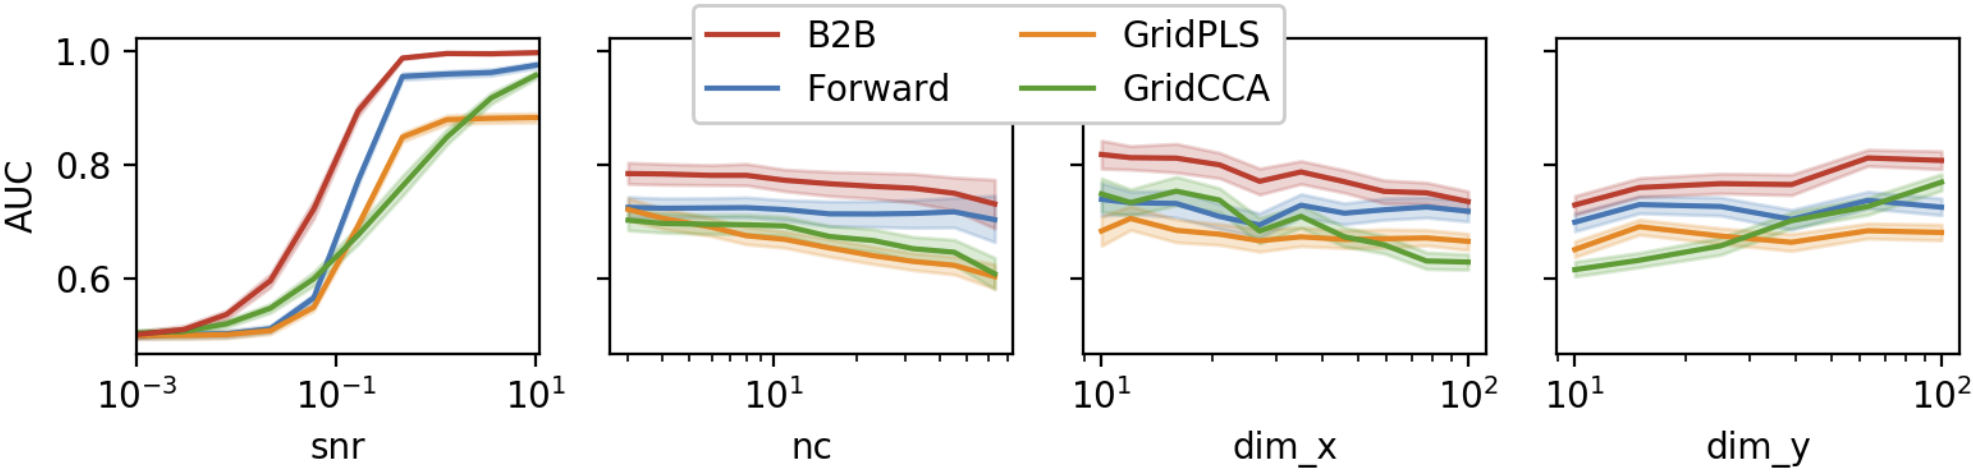
\includegraphics[width=\linewidth]{figures/AUC_conditions}
  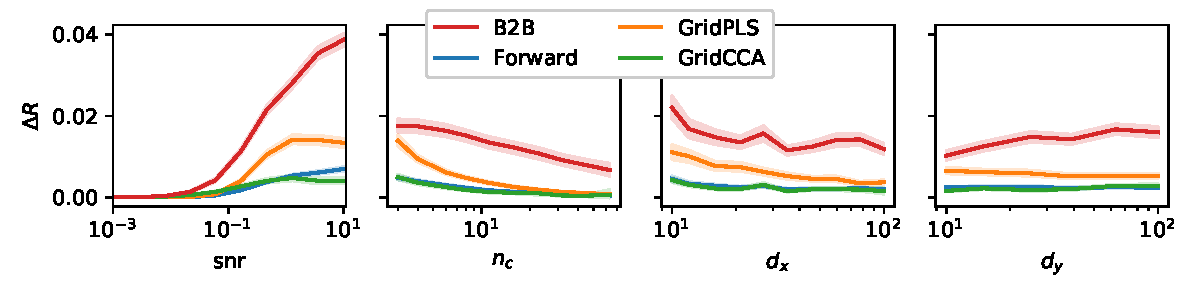
\includegraphics[width=\linewidth]{figures/R_conditions}
  \vspace{-4ex}
  \caption{Synthetic experiments. Average AUC (top) and Feature Importance $\Delta R$ (bottom) when varying experimental conditions individually. Higher is better. B2B compares favorably in all cases. \label{fig:percondition}}
\end{figure}


\subsection{Evaluating Causal Discovery with held-out prediction reliability}

In most cases, $E$ is not known and AUC can thus not be estimated.

To address this issue, we assess the ability of each model to reliably predict
independent and identically distributed data from $Y$, given all of the $X$
features versus all-but-ones feature $X_{-i}$ (i.e. 'knock-out X'). This procedure
results in two correlation metrics $R_{full}$ and $R_{knockout}$, whose
difference $\Delta R_i = R_{full}-R_{knockout}$ indicates how much each $X_i$
improves the prediction of $Y$.
%beyond what can be predicted from all other features $X_{-i}$.
In our figures, $\Delta R$ is the average of $\Delta R_i$. A higher score means that for prediction, the model relies on individual features rather than combinations of features.

We show in Appendix~\ref{appendix:feature_importance} pseudo-code to assess feature importance for our algorithm as well as baselines. For the Backward Model, feature importance cannot be assessed as there is no prediction.

% Feature importance can be computed similarly for the CCA, PLS and Forward baselines (see Appendix \ref{appendix:feature_importance}). For the Backward Model, feature importance cannot be assessed as there is no prediction.

We show in Figures~\ref{fig:percondition} (bottom) and \ref{fig:auc_plots} (right, in Appendix) that our method compares favorably to baselines.

%
% \iffalse
% For CCA and PLS, feature importance is assessed as follow:
% \begin{enumerate}
%   \item Fit $H$ and $G$ given $X_{train}$ and $Y_{train}$
%   \item For each feature $i$:
%   \begin{itemize}
%     \item Define $K$, and identity matrix whose row $i$ has been zeroed-out
%     \item Fit $H^i_k$ and $G_k$ given $X_{train} K$ and $Y_{train}$
%   \end{itemize}
% \end{enumerate}
% \fi
% For the Backward Model, feature importance cannot be assessed because there is no prediction.
% We thus simply
% report the model performance $R_i = corr(YG_i, X_i)$.


% \iffalse
% \begin{enumerate}
%
%   \item Fit $G$ given $X_{train}$ and $Y_{train}$
%   \item Fit $H$ given $X_{train}$ and $Y_{train} G^T$
%   \item For each feature $i$:
%   \begin{itemize}
%     \item Define $K$, and identity matrix whose row $i$ has been zeroed-out
%     \item Fit $H^i_k$ given $X_{train} K$ and $Y_{train} G^T$
%   \end{itemize}
%
%   \item Compute $R_{full}$ given $Y_{test} G^T$ and $X_{test}$
%   \item For all $i \in d_x$:
%   \begin{itemize}
%     \item Compute $R^i_{knockout}$ given $Y_{test} G^T$ and $X_{test} K {H^i_k}^T$
%     \item Compute $R^i_{delta}=R_{full} - R^i_{knockout}$
%   \end{itemize}
%   \end{enumerate}
% \fi

% \iffalse Ridge regression \citep{hoerl1959optimum}, multitask Lasso
% \citep{argyriou2008convex}, Partial Least Squares or PLS \citep{wold_pls,
% tenenhaus_pls}, Canonical Correlation Analysis or CCA \citep{cca_hotelling}, and
% Reduced Rank Regression or RRR \citep{Izenman_rrr}.
% %
% Each of these methods estimates a matrix of coefficients $\hat{W} \in
% \mathbb{R}^{d_x \times d_y}$, from which we estimate the diagonal mask $\hat{E}$
% using the feature importances $\hat{E}_{i,i} = \| W_{i, :} \|$.
% %
% For B2B, we obtain $\hat{E}$ as described in Algorithm~\ref{algorithm:b2br}.
% %
%
%
% We evaluate seven metrics:
% %
% test error in-distribution, test error out-distribution, test error-in
% distribution after weighting with $\hat{E}$, test error out-distribution after
% weighting with $\hat{E}$, Sonquist-Morgan false positives on $\hat{E}$,
% Sonquist-Morgan false negatives on $\hat{E}$, and the area under the ROC curve
% (AUC) between $\hat{E}$ and $E$.
% %
% The ``in-distribution'' metrics measure the test error of each predictor before
% and after weighting their features by the estimated (continuous!) mask
% $\hat{E}$.
% %
% The ``out-distribution'' metrics are similar, measuring the test error at
% samples drawn using two different random covariance matrices for both $X$ and
% $N$.
% %
% The false positives, false negatives, and AUC statistics measure the quality of
% identification of causal factors between $\hat{E}$ and the true, binary $E$.
%
% \begin{figure}[htpb] \centering
% 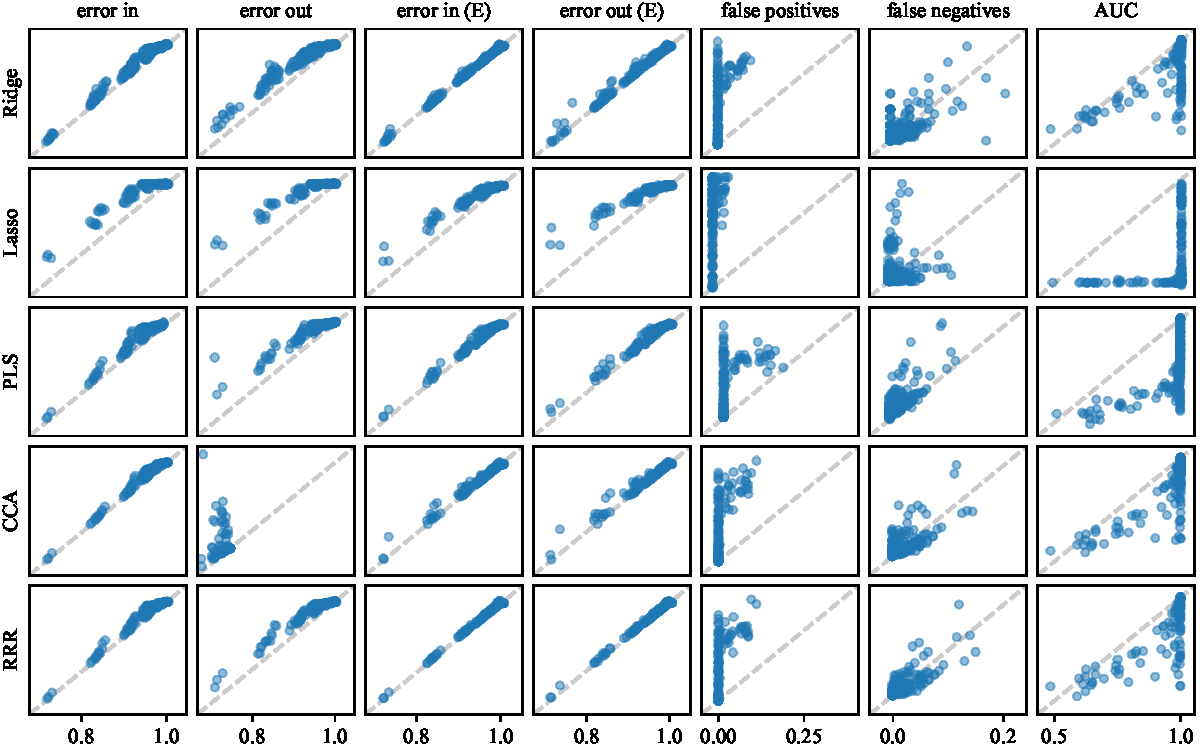
\includegraphics[width=\textwidth]{synthetic.pdf} \caption{Results of synthetic
% experiments. Each dot depicts the average value of a metric for B2B ($x$-axis)
% against a competitor ($y$-axis) for each experiment configuration averaged over
% $20$ random seeds. The prediction error on $Y$ within (in) and outside (out) of
% the training distribution are weakly but consistently larger for all of the
% models as compared to B2B with and without the Sonquist binarization (E). The
% AUC, measuring the ability of each model to separate causal from noncausal
% factors, is consistently larger in B2B as compared to the other models.}
% \label{table:synthetic} \end{figure} \fi

% Figure~\ref{table:synthetic} summarizes the results for all experimental
% conditions, metrics, and methods.
% %
% B2B is the method obtaining best test errors, lowest false positive and false
% negative discovery about $E$, and overall the best AUC when it comes to
% detecting causal influences.


\subsection{Magnetoencephalography data}
\label{sec:experiment_real}

%\newpage
%\subsection{Dataset}

Next, we apply our method to brain imaging data from the anonymized multimodal
neuroimaging ``Mother Of all Unification Studies'' (MOUS) dataset
\citep{schoffelen2019204}. The dataset contains magneto-encephalography (MEG)
recordings of 102 healthy native-Dutch adults who participated in a reading
task. Twelve subjects were excluded from the analysis because of corrupted file headers.
%
Subjects were exposed to a rapid serial visual presentation of Dutch words. The
word lists consisted of 120 sentences, and scrambled lists of the same words.
Each word was presented on the computer screen for 351ms on average (min: 300ms,
max: 1400ms). Successive words were separated by a blank screen for 300ms, and
successive sentences were separated by an empty screen for a few (3-4) seconds.

\subsubsection{MEG preprocessing}

The raw MEG data was bandpass-filtered between 0.1 and 40Hz using MNE-Python
default parameters \citep{gramfort2013meg, gramfort2014mne}. Specifically, we used a zero-phase finite impulse
response filter (FIR) with a Hamming window and with transition bands of 0.1Hz
and 10Hz for the low and high cut-off frequencies. The raw data was then segmented 100ms before word onset and 1s after
word onset ($t=0$ms corresponds to word onset). Finally, each resulting
segment was baseline-corrected between -100ms and 0ms, and decimated by 5 and
thus led a sampling frequency of 240Hz. The average responses across words is displayed in Figure \ref{fig:meg_evoked}.
For each subject and each time sample relative to word onset, we
build an observation matrix $Y \in \mathbb{R}^{n \times d_y}$ of $n\approx$ 2700 words
by $d_y=301$ MEG channels (273 magnetometers and 28 compensation channels). Each
of the columns of $Y$ is normalized to have zero mean and unit variance.

\begin{figure}[t!]
  \begin{minipage}[c]{0.6\textwidth}
    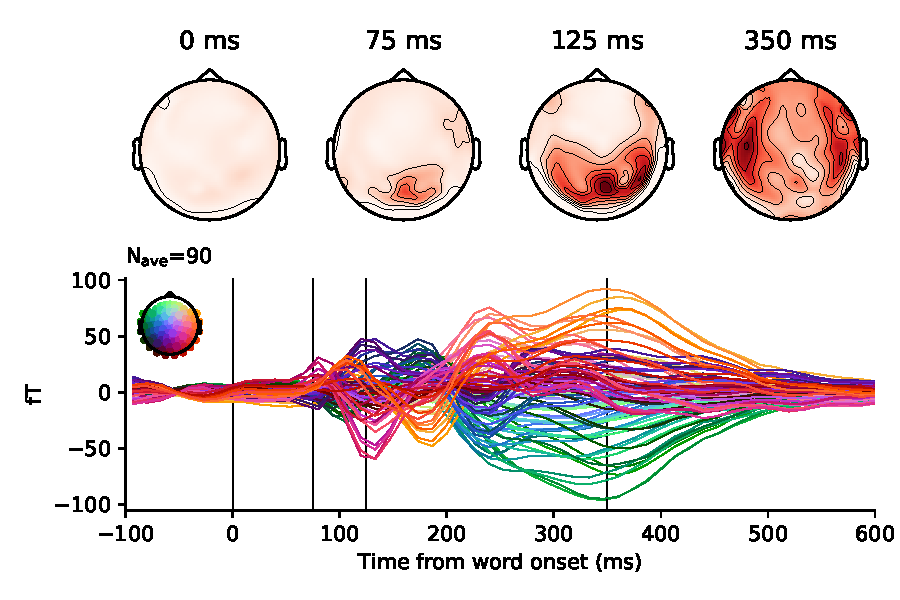
\includegraphics[width=\textwidth, trim=0cm 0cm 0cm 0cm, clip=True]{figures/meg_evoked.pdf}
  \end{minipage}\hfill
  \begin{minipage}[c]{0.4\textwidth}
    \caption{Ninety subjects read approximately 2,700 words while their brain activity was recorded with MEG. Top. Average brain response to words (word onset at t=0 ms), as viewed from above the head (red= higher gradient of magnetic flux). Bottom. Each line represents magnetometer, color-coded by spatial position. Posterior responses, typical of primary visual cortex activity, peak around 100 ms after word onset and are followed by an anterior propagation of activity typical of semantic processing in the associative cortices.
    }
    \label{fig:meg_evoked}
  \end{minipage}
\end{figure}


\subsubsection{Feature definition}

We aim to identify the word features that cause a variation in brain responses. We consider four distinct but colinear features.
%
First, 'Word Length' refers to the total number of letters. Word Length is expected to specifically cause a variation in the early evoked MEG responses (i.e. from 100 ms after stimulus onset) elicited by the retinotopically-tuned visual cortices (e.g. \citep{pegado2014timing}.).
%
Second, 'Word Frequency' indexes how frequently each word appears in Dutch and was derived with the the Zipf logarithmic scale of \citep{van2014subtlex} provided by the WordFreq package \citep{speerwordfreq}. Word Frequency is expected to specifically cause a variation in the late evoked MEG responses (i.e. from 400 ms), because it variably engages semantic processes in the temporal cortices \citep{kutas2011thirty}.
%
Third, 'Word Function' indicates whether each word is a content word (i.e. a noun, a verb, an adjective or an adverb) or a function word (i.e. a preposition, a conjunction, a determinant, a pronoun or a numeral), and was derived from Spacy's part of speech tagger \citep{spacy2}. To our knowledge, this feature has not been thouroughly investigated with MEG. Its causal contribution to reading processes in the brain thus remains unclear.
%
Finally, to verify that B2B and other methods would not inadequately identify non-causal features, we added a dummy feature, constructed from a noisy combination of Word Length and Word Frequency:
$dummy = z(length) + z(frequency) + \mathcal{N}$, where $z$ normalizes features and $\mathcal{N}$ is a random vector sampling Gaussian distribution (all terms thus have a zero-mean and a unit-variance).

This procedure yields an $X \in \mathbb{R}^{n \times d_x}$ matrix of $n\approx$ 2700 words by
$d_x=4$ features for each subject. Each of the columns of $X$ is normalized to
have a mean and a standard deviation of 0 and 1 respectively.

\subsubsection{Models and statistics}

We compare B2B to four standard methods: Forward regression, Backward regression, CCA and PLS, as implemented in scikit-learn \citep{sklearn}, and optimized with nested cross validation over twenty $l2$ regularization parameters logarithmically spaced between $10^{-4}$ and $10^4$ (for regression methods) or 1 to 4 canonical components (for cross-decomposition methods).

We used the feature importance described in Algorithm \ref{algorithm:b2b_fi} to assess the extent to which each feature $X_i$ specifically improves the prediction of held-out $Y$ data, using a 5-fold cross-validation.

Each model was implemented for each subject and each time sample independently. Pairwise comparison between models were performed using a Wilcoxon test across subjects (n=90) using the average $\Delta R$ across time.

Corresponding results are shown in Figure~\ref{fig:meg_results}.



\begin{wrapfigure}{r}{.5\textwidth}
  \vspace{-12ex}
  \begin{center}
    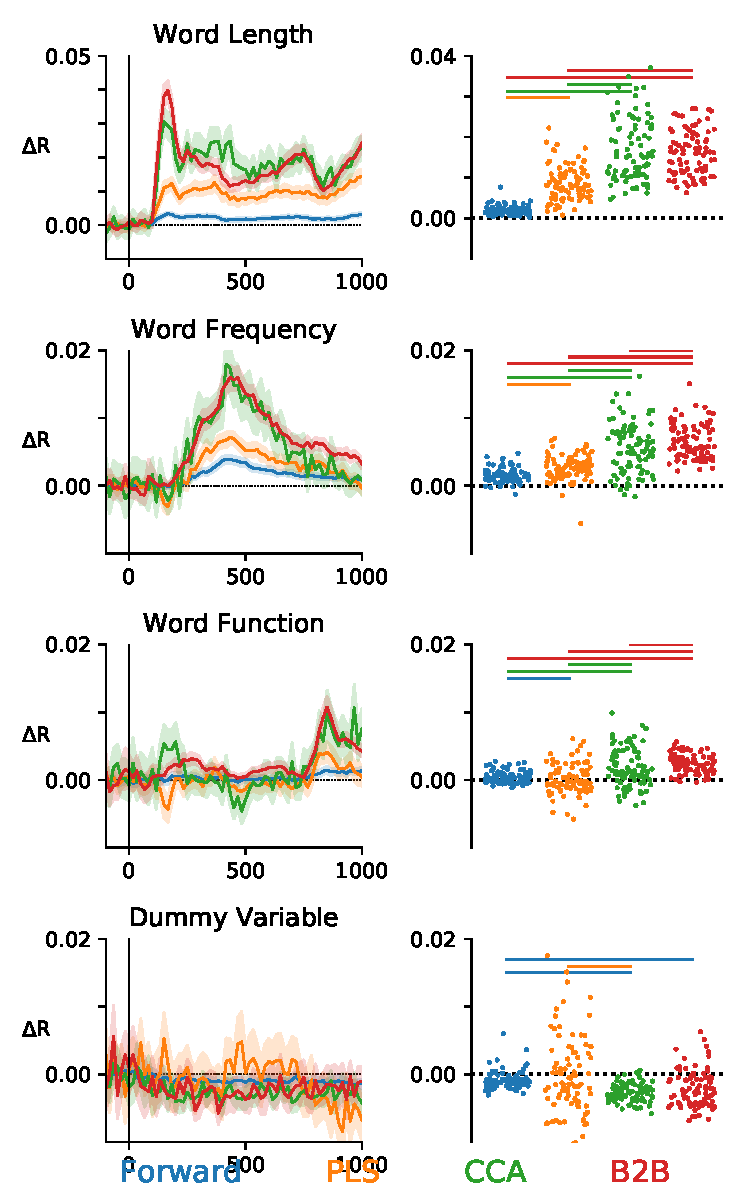
\includegraphics[width=0.48\textwidth, trim=0cm 0cm 0cm 0cm, clip=True]{figures/meg.pdf}

    \label{fig:meg_results}
  \end{center}
  \caption{Multiple models (color-coded) are compared on their ability to reliably predict single-trial MEG signals evoked by words. Left. Average improvement of correlation coefficient $\Delta R$ for each of the four features (rows). Error bars indicate standard error of the mean (SEM) across subjects. Right. Average $\Delta R$ across time for each subject (dot). Top horizontal lines indicate when B2B significantly outperforms other methods.}
  \vspace{-9ex}
\end{wrapfigure}

\subsubsection{Results}
We compared the ability of Forward regression, Backward regression, CCA, PLS and B2B to estimate the causal contribution of four distinct but collinear features on brain evoked responses to words.

Supplementary Figure \ref{fig:meg_supp} shows that the Backward model decodes the dummy variable well above chance level. In addition, the Backward model reveal a similar decoding time course for Word Length and Word Frequency, even though these features are known to specifically influence early and late MEG responses respectively \citep{kutas2011thirty}. These results illustrate that backward modelling cannot be used to estimate the causal contribution of collinear features.

We thus focus on the four remaining methods (i.e. Forward Regression, PLS, CCA, and B2B) and estimate their $\Delta R$ (i.e. the improvement of Y prediction induced by the introduction of a given feature into the model \ref{algorithm:b2b_fi}). Contrary to the Backward Model, none of the models predicted the Dummy Variable to improve the $Y$ prediction: all $\Delta R < 0$ (all $p > .089$).

Figure \ref{fig:meg_results} shows, for each model, the effects obtained across time (left) and subjects (right).

Word Length and Word Frequency improved the prediction performance of all methods: $\Delta R>0$ for all models (all $p<0.0001$). As expected, the time course associated with Word Length and Word Frequency rose from $\approx$ 100 ms and from $\approx$ 400 ms respectively. Furthermore, Word Function improved the prediction performance of all models (all $p < 0.0002$) except for PLS~($p=0.7989$). Overall, these results confirm that Word Length, Word Frequency and Word Function causally influence specific periods of brain responses to words.

To assess which model would be most sensitive to these causal discoveries, we compared B2B to other models across subjects (Figure \ref{fig:meg_results} right). For Word Length B2B outperforms all models (all $p < 0.00001$) but CCA ($p=0.0678$). For Word Frequency, B2B outperforms all models (all $p < 0.0006$). For "Word Function", B2B outperforms all models (all $p < 0.0015$). Overall, these results show that B2B reliably outperform standard methods, especially when the effects are difficult to detect.


\section{Related work}
% scholkopf2016modeling

Back-to-back regression is closely related to Canonical Correlation Analysis \citep{cca_hotelling}.
%
While CCA computes the eigenvector decomposition of \eqref{eq:solH}, while we compute its diagonal.
%
If \eqref{eq:solH} is diagonal, as in our model \eqref{eq:model}, the variables in $X$ are the eigenvectors.
%
If all the associated eigenvalues are either $0$ or $1$, then all the variables are either part of the $Y$ subspace, or orthogonal to it, respectively.
%
This is because these eigenvalues correspond to the squared cosine of the angle between the corresponding variable in $X$ and the $Y$ subspace.
%
Thus, back-to-back regression is equivalent to CCA under the constraint that the subspaces spanned by $X$ and $Y$ are perpendicular, $X$ is spanned by vectors of $Y$ and vectors orthogonal to $Y$, and that the parallel and orthogonal components of $X$ are spanned by disjoint sets of features of $X$.

There are, however, differences between CCA and back-to-back regression.
%
First, since our objective is not to characterise the proximity between $X$ and $Y$, but to measure causal influences, we can disregard the diagonalization of \eqref{eq:solH} performed by CCA.
%
Second, whereas CCA leverages all correlations between $X$ and $Y$, we filter some of them, through splitting and bagging.

B2BR is also related, but different, from usual causal discovery algorithms \citep{peters2017elements} that hypothesize on the direction of causality, or from measures of causal influence requiring time information \citep{granger1969investigating, janzing2013quantifying}.

\section{Conclusion}

In this work, we proposed Back-to-Back Regression (B2BR), a method to 
measure the causal influence of a potential set of variables generating some observations.
%
B2BR performs two successive multidimensional regressions: one from the output domain, and another one from the input domain.
%
We provided a theoretical guarantee about the consistency of B2BR, and compared it to several baselines in controlled synthetic experiments.
%
We also applied B2BR to a recent brain imaging dataset, analyzing the timing
of brain responses and their connection to word features.
%
We obtained results consistent with prior work in neuroscience literature, confirming the efficacy of B2BR for real data analysis.


% \section{Acknowlegements}
% Data were provided (in part) by the Donders Institute for Brain, Cognition and Behaviour.

\clearpage
\newpage

\bibliographystyle{plain}
\bibliography{paper}

%\section{Appendices}
%
%This should hold part of the tests, explanations on simulation, detailed results and stuff on meg data

\end{document}
